\chapter{General Methodology}
\label{cha:methods_applied_in_genetic_studies_on_humans}

The investigation of underlying genetic architecture of human traits is limited to non-experimental studies and one can broadly distinguish between two types: twin studies and association studies.
Twin studies make use of monozygotic and dizygotic twin pairs to estimate the contribution of genetic and environmental components of a trait.
In contrast, association studies make use of recently developed molecular methods to identify specific genetic variation within the human genome associated with a specific trait.
Within this section I will describe commonly used methods in both twin and molecular based association studies.
I will further describe methods used to estimate heritability and genetic correlations.

\section{Twin Studies}
\label{sec:twin_based_studies}

Twins have always been of special interest to scholars.
Indeed already Hippocrates has been reported to be interested in twins at around 5th century BCE\@.
While his original accounts are lost, the Roman politician and author Cicero described Hippocrates's observations of two ill brothers, suspected to be twins, with similar identical disease progression~\cite{Cicero44BC},
thus providing the first written account of a twin study.

Much later Francis Galton was one of the first persons to use twins in order to investigate the effect of genes and the environment on human behavior~\cite{Rende1990}.
However, only when~\citet{Simens1924} discovered the two distinct types of twins, namely \acrfull{mz} and \acrfull{dz} twins, twin studies became an established instrument in the investigation of genetic factors in humans.

MZ twins develop from a single fertilized egg and therefore share all of their genetic makeup.
On the other hand, \acrshort{dz} twins develop from two fertilized eggs and share only 50\% of segregating genetic variants.
This distinction forms the basis of all twin studies and allows use of structural equations relating observed trait and theorized underlying genetic and environmental effects.

In addition, genetic effects can be further distinguished between additive genetic effects (A) which represent the accumulated effect of all genetic variations and dominant (D) effects which represents interaction on the same genetic locus.
Environmental components are differentiated into shared environment (C) and unique environment (E).
Therefore, the total variance of any particular trait is $P = A+D+C+E$.

Since one can assume different correlations between MZ ($r_{MZ}$) and DZ ($r_{DZ}$) twin pairs one can estimate components of $P$.
While the correlations between twins within C and E are the same in both MZ and DZ twins, namely $1$ and $0$, respectively,
MZ twins have a correlation of $1$ for both A and D, while DZ pairs have a correlation of $\frac{1}{2}$ and $\frac{1}{4}$, respectively.
Therefore differences within MZ twins can be attributed to E alone.
Further, when we assume that DZ and MZ twins are exposed to the same degree of similarity within their environment, the differences in similarity between MZ and DZ twins is an estimate of all the genetic contribution to the phenotypic variance (i.e. including additive, dominant, and epistatic effects).
This is also called Falconer's formula (see Formula~\ref{eq:falcon}) and can be used to estimate broad sense heritability, also denoted as $H^2$:
\begin{align}
  H^2 &= 2(r_{MZ}-r_{DZ}) \label{eq:falcon} \\ 
  C &= r_{MZ} - H^2  \\
  E &= 1 - r_{MZ}  
\end{align}

However, while the above is attractive it its simplicity, today's twin studies use \acrfull{sem} to model genetic and environment effects.
SEM is more flexible in modeling specific hypotheses, such as testing for sex differences as well  handling multivariate data~\cite{Rijsdijk2002}.

Figure~\ref{fig:ace} displays such a classical path-based model.
Variables within a SEM can be separated into latent and observed variables.
Additive genetic (A), common environment (C) and unique environment (E) are  latent variables.
These variables are not directly observed but are inferred from actual measured variables.
Observed variables are commonly displayed in cornered boxes.
The double headed arrows represent the correlations among A and C.
The causal paths $a$, $c$, and $e$ represent the effect of the components on the trait $T$, and the square of these estimates represent the variance accounted for by each of the corresponding latent factors.
However, effects of $D$ cannot be simultaneously estimated with $A$, and two separate models need to be constructed.

\begin{figure}[htpb]
  \centering
  \scalebox{0.6}{%\usetikzlibrary{external}
%\tikzset{external/system call={latex \tikzexternalcheckshellescape -halt-on-error
%		-interaction=batchmode -jobname "\image" "\texsource";
%		dvips -o "\image".ps "\image".dvi ;
%		ps2eps "\image.ps" "\image".eps}}
%\tikzexternalize
%\newcommand{\at}{\makeatletter @\makeatother}
\begin{tikzpicture}[auto,node distance=.5cm,
    latent/.style={circle,draw,very thick,inner sep=0pt,minimum size=15mm,align=center},
    manifest/.style={rectangle,draw,very thick,inner sep=0pt,minimum width=45mm,minimum height=10mm},
    paths/.style={->, ultra thick, >=stealth'},
    twopaths2/.style={<->, ultra thick,bend left=90, >=stealth'},
    twopaths1/.style={<->, ultra thick,bend right=90, >=stealth'},
    mean/.style={draw, regular polygon, regular polygon sides=3, node distance=1cm, minimum height=15mm}
]

% Define observed variables
\node [manifest] (T1) at (0,0) {T1};
\node [manifest] (T2) [below=of T1, below=5cm of T1]  {T2};


% Define latent variables
\node [latent] (C1) [left=3.5cm of T1] {C1};
\node [latent] (C2) [left=3.5cm of T2] {C2};
\node [latent] (A1) [above=of C1] {A1};
\node [latent] (A2) [above=of C2] {A2};
\node [latent] (E1) [below=of C1] {E1};
\node [latent] (E2) [below=of C2] {E2};

\node [mean] (mu) at($(T1)!0.5!(T2)$)  {$\mu$};

% paths to T1/T2
\draw [paths] (A1.east) to node {$a$} (T1);
\draw [paths] (A2.east) to node {$a$} (T2);
\draw [paths] (C1.east) to node {$c$} (T1);
\draw [paths] (C2.east) to node {$c$} (T2);
\draw [paths] (E1.east) to node {$e$} (T1);
\draw [paths] (E2.east) to node {$e$} (T2);

% path from mean
\draw [paths] (mu.south) to node [right] {} (T2);
\draw [paths] (mu.north) to node [right] {} (T1);

% variance
\draw [twopaths1] (A1.west) to node  [bend left=90, left]{0.5 / 1} (A2.west);
\draw [twopaths2] (C2.west) to node  [bend right=90, left]{1} (C1.west);

\end{tikzpicture}
}
  \caption[ACE Model]{
    Basic ACE model.
    This basic model contains the latent variables A, C and E for twin 1 and 2, as well as the observed variable T with the mean $\mu$.
  }\label{fig:ace}
\end{figure}

The covariance matrix of the model in Figure~\ref{fig:ace} is therefore
\begin{equation}
  cov(MZ) = 
  \begin{pmatrix}
    a^2 + c^2 + e^2 & a^2 + c^2 \\
    a^2 + c^2 & a^2 + c^2 + e^2
  \end{pmatrix}
\end{equation}
and 
\begin{equation}
  cov(DZ) = 
  \begin{pmatrix}
    a^2 + c^2 + e^2 & \frac{1}{2}a^2 + c^2 \\
    \frac{1}{2}a^2 + c^2 & a^2 + c^2 + e^2
  \end{pmatrix}
\end{equation}
Modern SEM software are able to estimate parameters by minimising the goodness-of-fit statistic between the observed and predicted covariance matrices~\cite{Boker2011}.
Most commonly this is done via a maximum-likelihood function.
Furthermore, the overall goodness-of-fit of the model relative to a perfect fit, meaning that all covariances are estimated, is measured by a likelihood ratio square statistic ($\chi^2$).
Therefore, should we fail to reject the null hypothesis that our model in Figure~\ref{fig:ace} is different from a perfect fitted model we have reason to assume that our genetic model fits the data.

The use of SEM allows for great flexibility and a variety of models to be estimated.
In the past few decades numerous twin studies on a variety of traits have been performed.
It not only allowed testing for the differences in the genetic architecture between the sexes but also examining how influence of genetic factors change over age.
However, due to the new advances in molecular technology,  more research has  shifted to \acrfull{gwas}.
Hence, in the next section I will outline the methods applied in GWAS\@.

\section{Association Studies of Common Variants}
\label{sec:association_studies_of_common_variants}

Large-scale genomic association studies have enabled researchers to investigate specific genetic factors associated with a certain trait.
Hence, while twin studies were only able to give an estimate of the total contribution of genetic factors on a phenotype, association studies are able to elucidate the specific molecular basis of complex traits.
Specifically, these genome-wide association studies utilize common \acrfull{snp} and other genetic variants, to identify specific genetic markers associated with a certain trait.
Common variants are usually genetic variations with a frequency $\ge 1\%$, also called \acrfull{maf}.

\paragraph{What is a \acrfull{snp}}
\label{par:what_are_snp}
SNPs are variations within the genome at  specific positions and may underly differences in traits and disease susceptibility. 
For example, the replacement of the nucleotide cytosine (C) with thymine (T) at a certain position within a stretch of DNA is considered a \acrfull{snp}.

Association analysis of common genetic variants is usually only applied to investigate potential genetic markers of common traits and disorders, while different strategies are applied for rare diseases.
Indeed assessments of families whose members are disproportional affected with a rare genetic disorder, such as Huntigton's disease or cystic fibrosis, were able to identify a number of disease-causing variants~\cite{Kerem1989}.
However, while this method was initially successful with a number of other rare disorders, common disorders, such as heart disease, psychiatric disorders, as well as others, fared not that well,  
implying that common and rare disorders have a different genetic architecture~\cite{Hirschhorn2005a}.
This led to the development of the common disease common variant hypothesis.


\subsection{Common Disease Common Variant Hypothesis}
\label{sub:common_versus_rare_genetic_variants}

The common disease common variant hypothesis suggests that common disorders are affected by genetic variations which are also common in the population~\cite{Schork2010}.
This hypothesis, while simplistic, has some profound implications.

Importantly it is unlikely that common variants will have a high penetrance and are the lone disease-causing mutations.
For example, a common variant with a frequency of 45\% that directly causes a disorder would mean that also 45\% of the population would be affected by the disease.
This is unlikely to be the case and it is more likely that a given SNP only has a small effect on the disease.
This in turn also implies that multiple common variants affect a common disorder.
For example, twin studies have estimated the heritability of aggressive behavior at 50\%.
If a single SNP has only a small effect on the phenotype, then the total genetic risk must be distributed across multiple common genetic variants.
Figure~\ref{fig:rare_comon} displays the spectrum of genetic affects and allele frequency.
\begin{figure}[htpb]
  \centering
  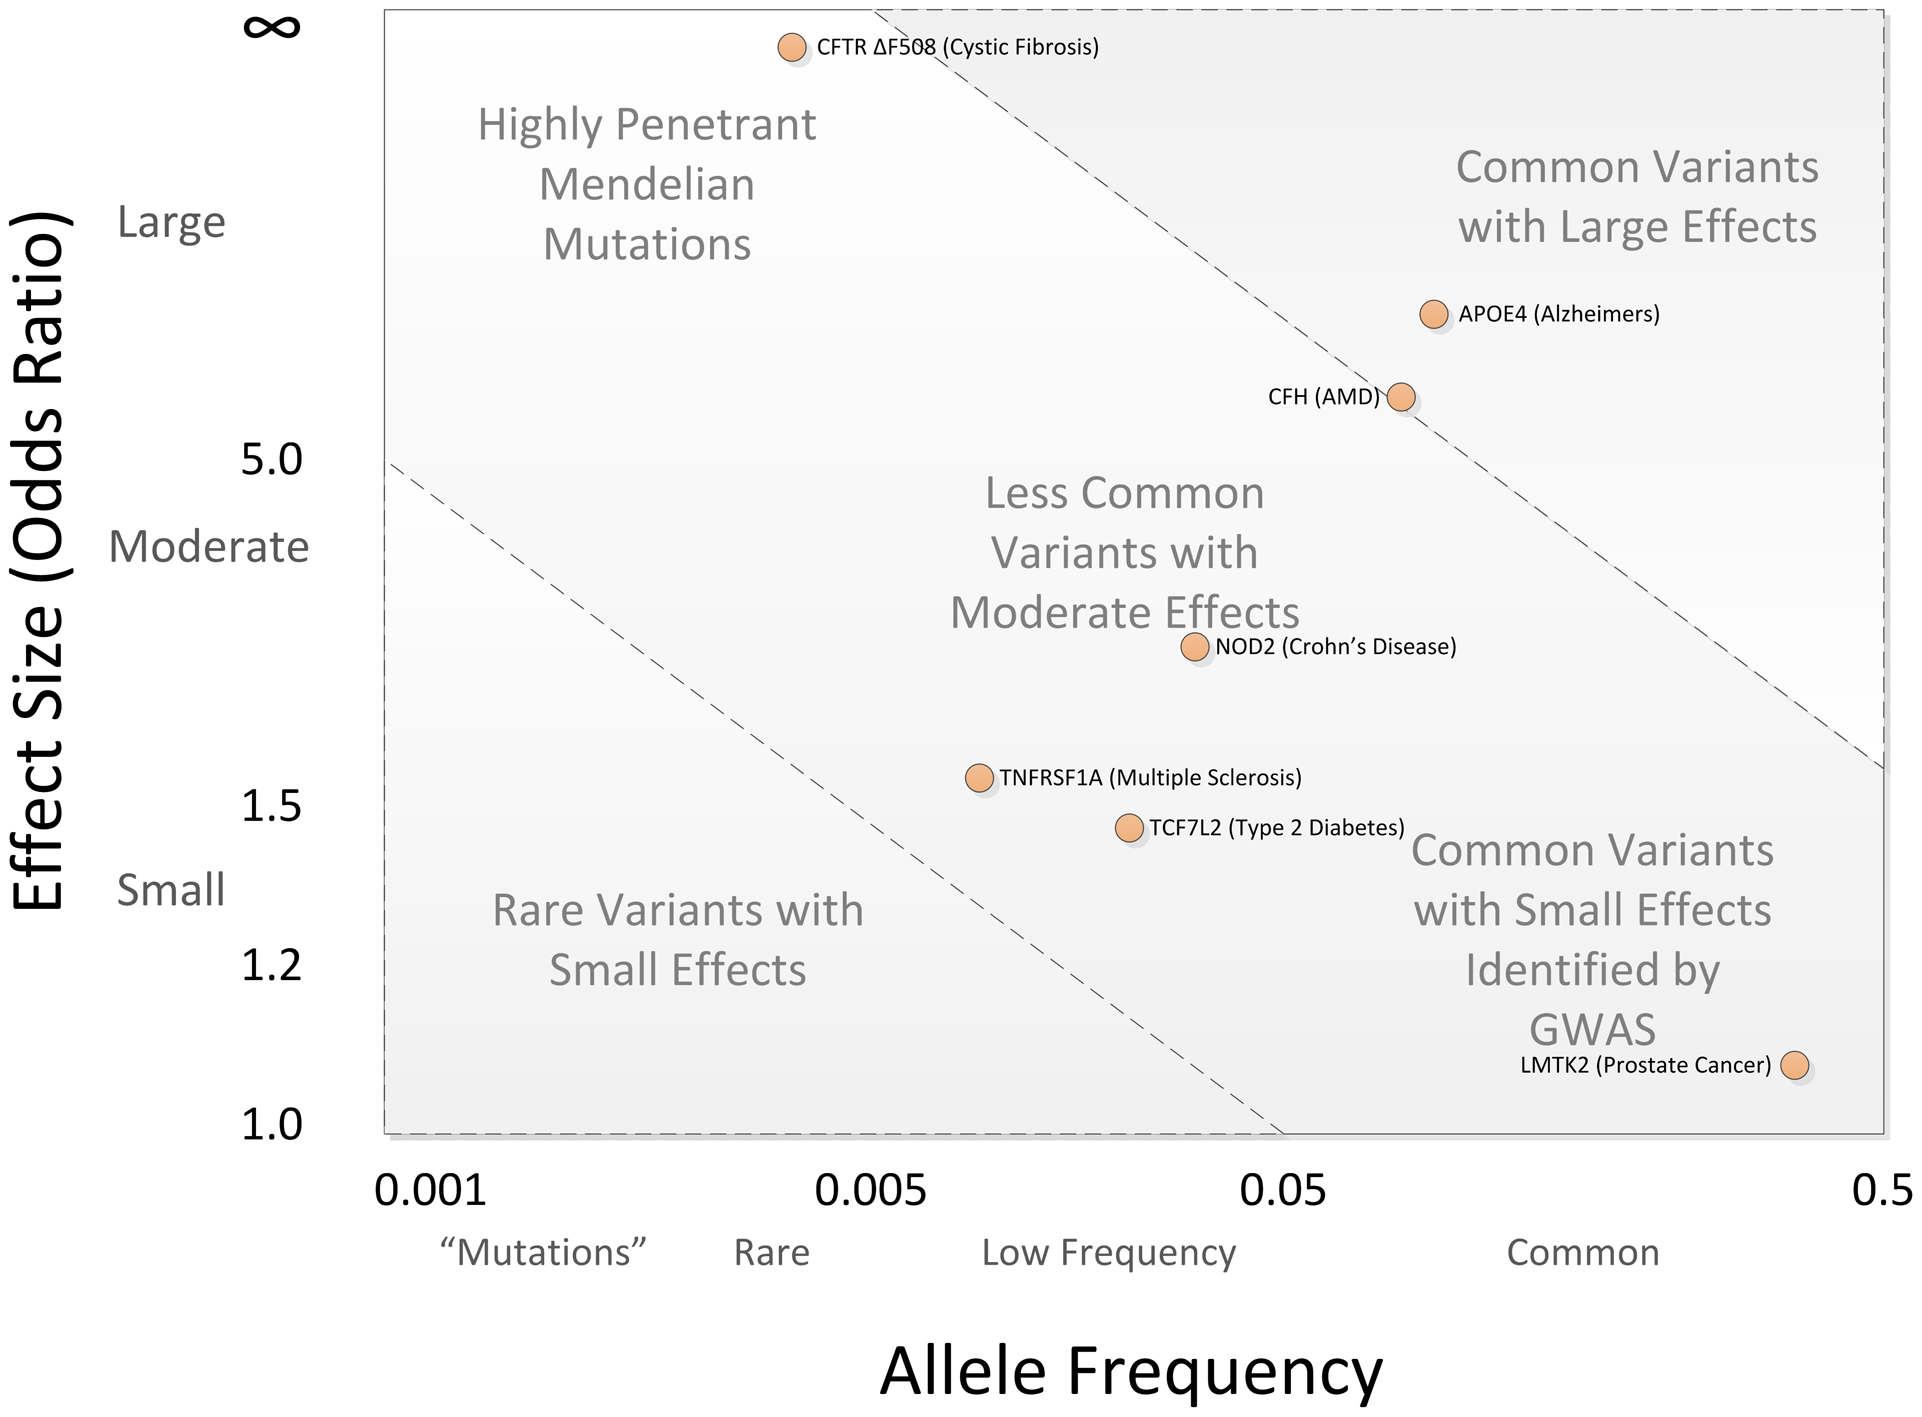
\includegraphics[width=0.8\linewidth]{{introduction/figure/journal.pcbi.1002822.g001}.png}
  \caption[Spectrum of Disease Allele Effects]{Spectrum of Disease Allele Effects~\cite{Bush2012}.}\label{fig:rare_comon}
\end{figure}

Overall, the common disease common variant hypothesis has been tested numerous times~\cite{Bush2012}.
Most common SNPs identified in the last 10 years are of small effect and most common disorders have multiple risk alleles~\cite{Welter2014,Schork2010}, suggesting that the hypothesis holds true. 
However this does imply that all genetic contributions to a common disorder are due to common variants alone.
Indeed, there have been some successful genetic associations of common variants in rare disorders.
For example,~\cite{Garcia-Barcelo2009a} identified 2 common SNPs associated with Hirschsprung's disease, a rare congenital disorder (2.8 per 10,000 births).

\subsection{Linkage Disequilibrium}
\label{sub:linkage_disequilibrium}

Before explaining the concept of association studies in more detail it is important to mention \acrfull{ld}.
LD is `the nonrandom association of alleles at different loci'~\cite{Slatkin2008} and forms a marker of the population genetic mechanism that is at play within our genome.
For example, two loci are said to be in high LD when allele $A$ at one loci co-occurs with allele $B$ at a different loci at a higher frequency then one would expect if the two loci were independent.
Hence the level of LD can be quantified as $D_{AB}=p_{AB} - p_{A}p_{B}$ in which in which $p_{AB}$ is the frequency that $A$ and $B$ occurs together wile $p_A$ and $p_B$ is the frequency of $A$ and $B$, respectively.
If $D_{AB} \neq 0$, A and B are said to be in linkage disequilibrium, otherwise the two alleles are in linkage equilibrium ($D_{AB}=0$).
Nevertheless, $D_{AB}$ depends on the frequencies of the alleles in questions and is therefore not always convenient.
Therefore, LD between two loci is commonly measured in two different ways. 
That is $D'$ and $r^2$.
\citet{Lewontin1964} suggested to use
\begin{equation}\label{eq:dprime}
  D' = D/D_{\min}
\end{equation}
where 
\begin{equation*}
  D_{\min}= \begin{cases}
    \max\{-p_A p_B,\,-(1-p_A)(1-p_B)\} & \text{when } D < 0\\
    \min\{p_A (1-p_B),\,(1-p_A) p_B\} & \text{when } D > 0
  \end{cases} 
\end{equation*}
Alternatively, one can also use the correlation coefficient $r$ between the two loci 
\begin{equation}\label{eq:r2}
  r=\frac{D}{\sqrt{p_A(1-p_A)p_B (1-p_B)}}
\end{equation}
An important consequence for association studies is that when an association between a trait and an allele is found, that allele is unlikely to be the actual causal SNP\@.
An association between a SNP and a trait can arise for multiple reasons.
First, the association could represent the true effect and the particular SNP has a causal relationship on the trait in question.
Second, and more likely, the associated SNP is a proxy of the causal SNP since both are in high \acrshort{ld}.
Third, the association is a random fluctuation within the sample, and 
fourth, the association is due to confounding errors such as population stratification or genotyping errors.

\subsection{Association Test}
\label{sub:association_test}

The association between a SNP $g$ and a trait $y$, as well as additional $p$ covariates $\bm{U}$, of an individual $i$ can be expressed as a generalized linear regression model for a continuous or binary phenotype:
\begin{equation}
  g(E(y_i)) = \beta_0 + \beta_1g_i + \bm{\beta_u}\bm{U_i'} + \epsilon
\end{equation}
in which $\beta_0$ is the intercept (commonly ignored in GWAS settings) and $\beta_1$ the regression coefficient of a particular SNP\@.
The vector $\bm{\beta_u}$ of size $1\times p$ are the regression coefficients of $p$ covariates to adjust for potential confounding factors.
Possible confounding factors are population stratification, sex, genotyping chip, and others.
The link function $g(.)$ is a logit function for binary traits, while for quantitative traits no transformation is used (identity link function). 

Genotypes of each SNP can be organized to represent dominant, recessive, multiplicative, as well as additive models~\cite{Bush2012}.
For example, assuming at a given position the two genotypes are \textit{A} and \textit{a}.
In a dominant model (for \textit{A}) having one or two copies of \textit{A} increases disease risk over no copies of \textit{A}.
Thus the risk $k$ is the same for \textit{Aa} and \textit{AA}.
In contrast, a recessive model (for \textit{A}) requires at least two copies of the risk allele \textit{A}.
The multiplicative model (for \textit{A}) assumes a quadratic increase in risk.
If the risk of having the \textit{A} allele is $k$ than having two copies of the same allele is $k^2$.
An additive model assumes a linear increase in risk for each additional allele copy.
Thus if the risk of \textit{Aa} is $k$ then the risk doubles ($2k$) for \textit{AA}. 
Despite these different models, GWAS commonly uses an additive model only since it has appropriate statistical power to detect dominant effects as well.
Nevertheless, it is important to keep in mind that an additive model has reduced power for potential recessive effects~\cite{Bush2012}.

\subsection{Population Stratification}
\label{ssec:population_stratification}

Population stratification takes place when differences in the frequencies of alleles among cases and controls are not due to a causal relationship between the SNP and the trait.
Rather, they are caused by ancestral differences across populations.
An association is affected by population stratification if the trait is more prevalent in one population while the allele frequencies vary across the populations.

Commonly one can adjust for population stratification by the usage of \acrfull{pca}.
PCA is a procedure which transforms a set of correlated variables into a set of linear uncorrelated ones, called principle components (\acrshort{pc}).
The number of PC can be smaller or equal to that of the number of initial variables and the first PC accounts for most of the variability in the set of correlated variables.
Each following PC explains the most variance constrained that it is orthogonal to the previous.

Using PCA on a matrix of individuals by SNPs, in which each cell represents the count of minor alleles, results in a set of PCs which explain the genetic variation within the sample.
Given the sample is a mixture out of multiple populations with different ancestry the computed PCs will often have geographic interpretation.
Thus including PCs into the association model will adjust for population stratification arising due to differences in allele frequencies and disease prevalence.

\subsection{Multiple Testing}
\label{ssec:multiple_testing}

Testing a large number of genetic variants without adjusting the significance threshold $\alpha$ results in a large number of falsely associated variants.
Therefore, adjustment of the significance threshold is necessary.
For example, one could simply adjust $\alpha$ by the number of tests performed (Bonferroni threshold).
However, this would result in an overly conservative threshold and in a number of false negative associations~\cite{Benjamini1995} since computed test statistics are not independent due to LD\@.
Indeed,~\citet{Peer2008} estimated, based on data from the International Haplotype Map Consortium, the number of independent tests to be one million in Europeans and two million in African populations.
Therefore most GWAS have used a threshold of $5\times 10^{-8}$.
However, due to the introduction of larger sample sizes as well as better technology we are able to genotype variants with lower allele frequency.
This requires more stringent adjustment of the GWAS significant threshold since it also increases the number of independent tests.
Hence~\citet{Fadista2016} recently suggested to use $3\times10^{-8}$, $2\times10^{-8}$, $1\times10^{-8}$ when including variants with $MAF\ge1\%$, $MAF\ge0.5\%$, and $MAF\ge0.1\%$, respectively.

\acrshort{gwas} are useful in identifying molecular markers for traits and diseases.
While there are multiple possible confounding factors, such as population stratification, methods have been developed to approach these problems successfully.


\section{Heritability and Genetic Correlation}
\label{sec:heritability_and_genetic_correlation}

As already described above, studies on twins were able to assess the heritability of traits by considering the MZ and DZ twin correlations.
Interestingly, a number of methods have also been developed to assess narrow sense heritability, or the additive genetic effect, from genotyped data.
Several methods have been proposed in the past, most notably \acrfull{gcta} and LD-score regression.

\subsection{\acrfull{gcta}}
\label{sub:gcta}

GCTA uses a mixed linear model to  fit the effect of all SNPs by making use of the genetic relationship matrix of all included subjects~\cite{Yang2011}.
If $\textbf{A}$ is the genetic relatedness matrix then
\begin{equation}
  y = X\beta + g + \epsilon \text{ with } var(y) = V = A\sigma^2_g + I\sigma^2_\epsilon
\end{equation}
in which $y$ is the phenotype and $\beta$ are the estimated effect sizes of all covariates and the total genetic effect $g$ for each individual is $g \sim N(0, A\sigma^2_g)$.
GCTA is then able to estimate the variance explained by all SNPs, $\sigma^2_g$, by restricted maximum likelihood.
One can extent this model to bivariate linear mixed models to estimate the genetic correlation between two traits as well.
If $y_1 = X_1\beta_1 + g_1 + \epsilon_1$ for trait 1 and $y_2= X_2\beta_2 + g_2 + \epsilon_2$ for trait 2 then the variance-covariance matrix $V$ is
\begin{equation}
  V = 
  \begin{pmatrix}
    Z_1AZ_1'\sigma_{g1} + I\sigma^2_{\epsilon 1} & Z_1AZ_2'\sigma_{g_1g_2} \\
    Z_2AZ_1'\sigma_{g_1g_2} & Z_2AZ_2'\sigma_{g2} + I\sigma^2_{\epsilon 2}
  \end{pmatrix}
\end{equation}
in which $X$ and $Z$ are the incidence matrices for the effects of $\beta$ and $g$.
However, GCTA requires considerable computational power as well as the availability of the raw genotype data.
Hence LD-score regression has been developed to estimate heritability on summary statistics only.

\subsection{LD-score Regression}
\label{sub:ld_score_regression}

LD-score regression makes use of the previously outlined LD among tagged and causal SNPs.
Test statistics of SNPs in high LD with the causal variant will be elevated proportional to their LD\@.
Thus the more genetic variation a SNP tags the higher the probability that it will tag a causal variant.
LD-score regression makes use of this relationship and regresses the estimated $\chi^2$ from the association study on the LD-score, which measures the overall LD of variant $j = 1, \ldots, M$ as $\ell_j = \sum^M_{k=1} r^2_{jk}$. 
The slope of this regression can then be interpreted as an estimate of heritability~\cite{Bulik-Sullivan2015}.
Similarly, if we replace the $\chi^2$ of a single study by the product of the z-scores of two separate studies and regress it onto $\ell_j \sqrt{N_{1}N_{2}}$, the slope can be interpreted as the genetic covariance between trait 1 and 2~\cite{Bulik-Sullivan2015a}.

\section{The Missing Heritability}
\label{sec:missing_heritability}

One would expect that the variance explained by all genetic variants combined would result in similar estimates as to those estimated in twin studies.
Unfortunately, for many traits, this is not the case.
This is called the `Missing Heritability Problem'~\cite{Vineis2010} and a  number of reasons have been suggested for the discrepancy between estimates in twin studies and those in GWAS\@.

First, the assumptions in twin studies might be violated and estimates are too high.
In particular, studies on twins assume that shared environmental factors influence MZ and DZ twins to the same extent.
However, one can argue that MZ twins are treated by parents, teachers, and peers differently resulting in a potential violation of the this equal environments assumption. 
However, while previous research suggest that the equal environment assumption might not be strictly valid, the induced bias is likely to be small~\cite{Derks2006,Felson2014}

Second, GWAS only consider common variants and rare variants might account for the missing heritability.
While most rare variants have little or no effect on traits, some rare variants have very large effects.
Indeed, a study on height found that while most common variants only had small effects, some rare genetic variants resulted in a large increase in height of up to $2cm$~\cite{Marouli2017}.
This would indicate that rare variants can have a profound effect on common traits, suggesting that heritability estimates using common variants alone might be biased downward.

Third, epistasis is only insufficiently captured in most studies and could account for the differences.
Indeed, many twin concordance rates indicate the presence of non-additive effects to some extent.
Further, complex gene-gene interaction have been shown in a number of experimental studies in  animals~\cite{Zuk24012012}.
Therefore suggesting that epistatic effects might play a major role in humans as well.
However, models which include gene-gene or even gene-gene-gene and higher order interactions are very computational intensive and require large datasets~\cite{Lippert2013}. 

Fourth, gene regulatory components, such as RNA expression and methylation, might explain the discrepancy between estimates.
Methods investigating regulatory components have only been recently introduced for large-scale population analysis and alteration of gene expression by epigenetic modifications could be heritable without affecting the underlying DNA sequence~\cite{Trerotola2015,Nadeau2009}.
Indeed, various studies have shown that some environmental factors can lead to epigentic changes that can be carried over to following generations without continued exposure~\cite{Nadeau2009,Skinner2011}.
This separate model of inheritance, next to Mendelian heredity, would be undetectable in GWAS\@.

While a single reason for the missing heritability seems unlikely it is still an ongoing research objective to account for the differences.

\subsection{Genetic Correlations}
\label{sub:genetic_correlations_method}
The development of both LD-score regression and GCTA have enabled recent research to uncover the genetic correlations among a variety of different traits, even when the two traits are measured on different people.
However, genetic correlation can arise from a multitude of different sources.
Figure~\ref{fig:genetic_correlation} shows 4 different ways genetic correlation can arise.
First and foremost, genetic correlation can arise if two traits are caused by the same genetic factors (see Figure~\ref{fig:pleiotropy}).
Second, a genetic factor  causes phenotype 1 and that phenotype can in turn cause phenotype 2 (see mediated pleiotropy in Figure~\ref{fig:mediated_pleiotropy}).
Third, genetic correlation can also arise from assortative mating as shown in Figure~\ref{fig:assortative_mating}.
Assortative mating is a non-random mating pattern within a population.
For example, consider two traits which share no causal variant.
Trait 1 is desirable in males while trait 2 is desirable in females.
Over a few generation this will result in LD between causal variants of trait 1 and 2 despite sharing no initial causal SNPs, resulting in a genetic correlation. 
Fourth, also parental effect can result in genetic corrections as displayed in Figure~\ref{fig:parental_effects}.
Specifically, genetic components cause trait $1$ in the parents which influences the child's environment which in turn results in trait 2. 
Nevertheless, the genetic correlations estimated by LD-score and GCTA are unable to distinguish between the possible sources of genetic correlations.

\begin{figure}[htp]
  \begin{subfigure}[t]{0.4\textwidth}
    \centering
    \resizebox{0.5\linewidth}{!}{\begin{tikzpicture}[auto,node distance=.5cm,
    latent/.style={circle,draw,very thick,inner sep=0pt,minimum size=10mm,align=center},
    manifest/.style={rectangle,draw,very thick,inner sep=0pt,minimum width=45mm,minimum height=10mm},
    paths/.style={->, ultra thick, >=stealth'},
    twopaths2/.style={<->, ultra thick,bend left=90, >=stealth'},
    twopaths1/.style={<->, ultra thick,bend right=90, >=stealth'},
    mean/.style={draw, regular polygon, regular polygon sides=3, node distance=1cm, minimum height=10mm}
]

\node [latent] (G) at (0,0) {G};
\node [latent] (P1) at (-2,-2) {P1};
\node [latent] (P2) at (2,-2) {P2};

\draw [paths] (G.south west) to node [right] {} (P1);
\draw [paths] (G.south east) to node [right] {} (P2);

\end{tikzpicture}
} 
    \caption{Pleiotropy}\label{fig:pleiotropy}
  \end{subfigure}
  \begin{subfigure}[t]{0.4\textwidth}
    \centering
    \resizebox{0.5\linewidth}{!}{\begin{tikzpicture}[auto,node distance=.5cm,
    latent/.style={circle,draw,very thick,inner sep=0pt,minimum size=10mm,align=center},
    manifest/.style={rectangle,draw,very thick,inner sep=0pt,minimum width=45mm,minimum height=10mm},
    paths/.style={->, ultra thick, >=stealth'},
    twopaths2/.style={<->, ultra thick,bend left=90, >=stealth'},
    twopaths1/.style={<->, ultra thick,bend right=90, >=stealth'},
    mean/.style={draw, regular polygon, regular polygon sides=3, node distance=1cm, minimum height=10mm}
]

\node [latent] (G) at  (0,0) {G};
\node [latent] (P1) at (2,0) {P1};
\node [latent] (P2) at (4,0) {P2};

\draw [paths] (G.east) to node [right] {} (P1);
\draw [paths] (P1.east) to node [right] {} (P2);

\end{tikzpicture}
} 
    \caption{Mediated Pleiotropy}\label{fig:mediated_pleiotropy}
  \end{subfigure}
  \begin{subfigure}[t]{0.4\textwidth}
    \centering
    \resizebox{0.6\linewidth}{!}{
\begin{tikzpicture}[auto,node distance=.5cm,
    latent/.style={circle,draw,very thick,inner sep=0pt,minimum size=10mm,align=center},
    manifest/.style={rectangle,draw,very thick,inner sep=0pt,minimum width=45mm,minimum height=10mm},
    paths/.style={->, ultra thick, >=stealth'},
    paths2/.style={<->, ultra thick, >=stealth'},
    twopaths2/.style={<->, ultra thick,bend left=90, >=stealth'},
    twopaths1/.style={<->, ultra thick,bend right=90, >=stealth'},
    mean/.style={draw, regular polygon, regular polygon sides=3, node distance=1cm, minimum height=10mm}
]

\node [latent] (P2) at (0,0) {P2};
\node [latent] (P1) at (2,0) {P1};

\node [latent] (G1) at (5,0) {G1};
\node [latent] (G2) at (-3,0) {G2};

\node [latent] (E1) at (4,2) {E};
\node [latent] (E2) at (-2,2) {E};

\node [latent] (P1c) at (2,-2) {P1};
\node [latent] (P2c) at (0,-2) {P2};

\node [latent] (G1c) at (5,-2) {G1};
\node [latent] (G2c) at (-3,-2) {G2};

\node [latent] (E1c) at (4,-4) {E};
\node [latent] (E2c) at (-2,-4) {E};

\draw [paths] (P1.east) to node [right] {} (G1);
\draw [paths] (P2.west) to node [right] {} (G2);
\draw [paths] (G1.south) to node [right] {} (G1c);
\draw [paths] (G2.south) to node [right] {} (G2c);
\draw [paths] (E1.south west) to node [right] {} (P1);
\draw [paths] (E2.south east) to node [right] {} (P2);

\draw [paths] (G1c.west) to node [right] {} (P1c);
\draw [paths] (G2c.east) to node [right] {} (P2c);

\draw [paths] (E1c.north west) to node [right] {} (P1c);
\draw [paths] (E2c.north east) to node [right] {} (P2c);

\draw [paths2] (P1.west) to node [right] {} (P2.east);


\node [text width=1cm] at (5,1) {Father};
\node [text width=1cm] at (-3,1) {Mother};
\node [text width=1cm] at (-3,-3) {Child};

\end{tikzpicture}
} 
    \caption{Assortative Mating}\label{fig:assortative_mating}
  \end{subfigure}
  \begin{subfigure}[t]{0.4\textwidth}
    \centering
    \resizebox{0.6\linewidth}{!}{\begin{tikzpicture}[auto,node distance=.5cm,
    latent/.style={circle,draw,very thick,inner sep=0pt,minimum size=10mm,align=center},
    manifest/.style={rectangle,draw,very thick,inner sep=0pt,minimum width=45mm,minimum height=10mm},
    paths/.style={->, ultra thick, >=stealth'},
    twopaths2/.style={<->, ultra thick,bend left=90, >=stealth'},
    twopaths1/.style={<->, ultra thick,bend right=90, >=stealth'},
    mean/.style={draw, regular polygon, regular polygon sides=3, node distance=1cm, minimum height=10mm}
]

\node [latent] (Gp) at (0,0) {G};
\node [latent] (P1) at (2,0) {P1};
\node [latent] (Ep) at  (4,0) {E};
\node [latent] (Gc) at (0,-2) {G};
\node [latent] (Ec) at  (2,-2) {E};
\node [latent] (P2) at (4,-2) {P2};

\node [text width=1cm] at (-1.5,0) {Parent};
\node [text width=1cm] at (-1.5,-2) {Child};

\draw [paths] (Gp.east) to node [right] {} (P1);
\draw [paths] (Gp.south) to node [right] {} (Gc);
\draw [paths] (P1.south) to node [right] {} (Ec);
\draw [paths] (Ep.west) to node [right] {} (P1);
\draw [paths] (Ec.east) to node [right] {} (P2);

\end{tikzpicture}
}
    \caption{Parental Effects}\label{fig:parental_effects}
  \end{subfigure}
  \caption[Sources of Genetic Correlations]{Different sources of genetic correlation according to~\citet{Pickrell2016}}\label{fig:genetic_correlation}
\end{figure}

To conclude, during the last few years large gains have been made in fostering our understanding of heritability and genetic correlations with the development of GCTA and LD-score regression.
While these tools are able to estimate heritability and genetic correlations of a number of traits it remains difficult to distinguish between different sources of genetic correlations.

\section{Association Studies on Rare Variants}
\label{sec:association_studies_on_rare_varitants}

A possible suspect for the missing heritability are rare variants.
Rare variants,  variants with a \acrfull{maf} of 1\% or lower, have been suggested to explain the bulk of missing heritability~\cite{Jiang2013,Li2009a}.
Rare variants are commonly not accessible via micro array chips but only via the more cost intensive sequencing.
However, the drop in sequencing costs has allowed us to conduct whole-exome and whole genome association studies of rare variants~\cite{Goodwin2016}.
In contrast to GWAS, single variant associations are largely unfeasible, unless sample size is very large~\cite{Lee2014}.
Hence, considerable effort has been made to develop and deploy statistical methods to improve statistical power of rare variant association studies~\cite{Morris2010,Zeng2014,Daye2012,Manuscript2013}.
Instead of testing individual genetic markers most statistical tests evaluate the combined effect of multiple genetic variations in a biologically-relevant region, such as a gene.
In general, one can divide such approaches into burden and variance component tests.
I will first introduce the general statistical model for the two tests.
Following, I will outline two commonly used classes of tests and evaluate their benefits and drawbacks.

Assuming that $y_i$ for subject $i$ with mean $\mu_i$ follows a distribution in the quasi-likelihood family~\cite{Lee2014} with $n$ subjects in a region with $m$ variants, then
\begin{equation}
  h(\mu_i) = \alpha_0 + \alpha'X_i +\beta'G_i
\end{equation}
in which $h(\mu) = \mu$ or $h(\mu) = logit(\mu)$.
The regression coefficients of the covariates and allele counts are $\alpha = (\alpha_1, \ldots, \alpha_q)$ as well as $\beta = (\beta_1, \ldots, \beta_m)$, respectively.
The covariates are denoted as $X_i = (X_{i1}, \ldots, X_{iq})'$ and the allele counts as $G_{i1}, \ldots, G_{im}$.
The score statistic of the marginal model for variant $j$ is then
\begin{equation}
  S_j = \sum^n_{i=1} G_{ij}(y_i-\hat{\mu_i})
\end{equation}
where $\hat{\mu_i}$ is the estimated mean under $H_0: \beta = 0 $ and is obtained by $h(\mu_i) = \alpha_0 + \alpha'X_i$.

\subsection{Burden Test}
\label{sub:burden_test}
The simplest approach, called the burden test, tests the weighted sum of computed scores:
\begin{equation}\label{eq:burden}
  Q = {(\sum^{m}_{j=1} w_{j} S_{j})}^2
\end{equation}
in which $w_j$ is the weight for variant $j$.
Weights can be define by functional annotations, allele frequency, or other means.
The test assumes that all variants  have the same direction of effect.
This is a rather strong assumption and violations result in a loss in statistical power~\cite{Derkach2013a}.

\subsection{Variance Components Tests}
\label{sub:variance_component_tests}
In contrast to burden tests, variance-components tests evaluate the distribution of effects within a certain genomic region.
The most prominent member of this test family is \acrfull{skat}~\cite{Wu2011}.
SKAT assumes that $\beta_j\sim N(0,w_j\tau)$ and tests for $H_0: \tau = 0$ with a variance-components score test.
The test statistic is defined as
\begin{equation}\label{eq:skat}
  Q = \sum^{m}_{j=1} w_{j}^2 S_{j}^2
\end{equation}
The test is robust to groupings of protective and damaging effects within the same region.
However,  SKAT suffers from a reduction in statistical power in cases of high proportions of causal variants of the same direction, as compared to the burden test~\cite{Derkach2013a}.

To summarise, variance-components tests are generally more powerful than burden tests if a region has many non-causal variants or when the effects of a genomic region are bi-directional.
In contrast, burden tests perform better in scenarios where most causal variants have the same direction of effect.
This has led to the development of omnibus tests to combine burden and variance component tests, most notably SKAT-O~\cite{Lee2012}.
\bigskip

To conclude, I have outlined various statistical methods to investigate the genetic contribution of aggressive behavior.
I have described the commonly applied twin model to estimate the contribution of genetic and environmental effects.
Further, I outlined the principles of genome wide association studies as well as the use of GCTA and LD-score to estimate the narrow sense heritability from common SNPs.
Finally, I have described two commonly-used rare variant tests as well as their pros and cons.

In the next chapter I will present an investigation of the longitudinal heritability of childhood aggression with the use of two large twin cohorts. 
